\documentclass{article}
\usepackage{amsmath, graphicx, import, cancel}
\usepackage{amsthm, xcolor, caption, subcaption}
\author{Apisit Thaweboon \: 65050988}
\date{}
\title {\textbf{
        SEPERABLE DIFFERENTIAL
    }
}
\begin{document}

\section*{Introduction to SP}
\begin{align}
\begin{split}
    \frac{dy}{dx} = g(x)f(y) \\
    h(y) = \frac{1}{g(y)} \\
    \frac{dy}{dx} = \frac{g(x)}{h(y)} \\
    \frac{h(y)}{dy} = \frac{g(x)}{d(x)} \\
    \frac{dy}{dx} = \frac{x^2}{y^2} \\
    \text{Draw directinal field} \\
\notag
\end{split}
\end{align}


\section*{second ex}
\begin{align}
\begin{split}
    \frac{dy}{dx} = \frac{6x^2}{2y + \cos{y}} \\
    \int{(2y + \cos{y}) }dy = \int{6x^2}dx \\
    y^2 + \sin{y} = 2x^3 + c \\
\notag
\end{split}
\end{align}


\section*{Third ex}
\begin{align}
\begin{split}
    y' &= x^2y \\
    \frac{dy}{dx} &= x^2y \\
    \int{dy}{y} &= \int{x^2}dx \\
    \ln{|y|} &= \frac{1}{3}x^3 + c \\
    e^{\ln{|y|}} &= e^{\frac{1}{3}x^3 + c} \\
    |y| &= Ae^{\frac{1}{3}x^3} \\
    \text{this is not function due to \abs{y}, this is relation} \\
\nonumber
\end{split}
\end{align}


\section*{ex 4}
\begin{align}
\begin{split}
    \frac{dy}{dx} = \frac{x^2}{y^2} \\
    \int{y^2}dy = \int{x^2}dx \\
    \frac{1}{3}y^3 = \frac{1}{3}x^3 + c \\
    y = \sqrt{3}{x^3 + c} \\
\notag
\end{split}
\end{align}
\begin{figure}[h!]
    \centering
    \begin{subfigure}[b]{0.4\textwidth}
        \centering
        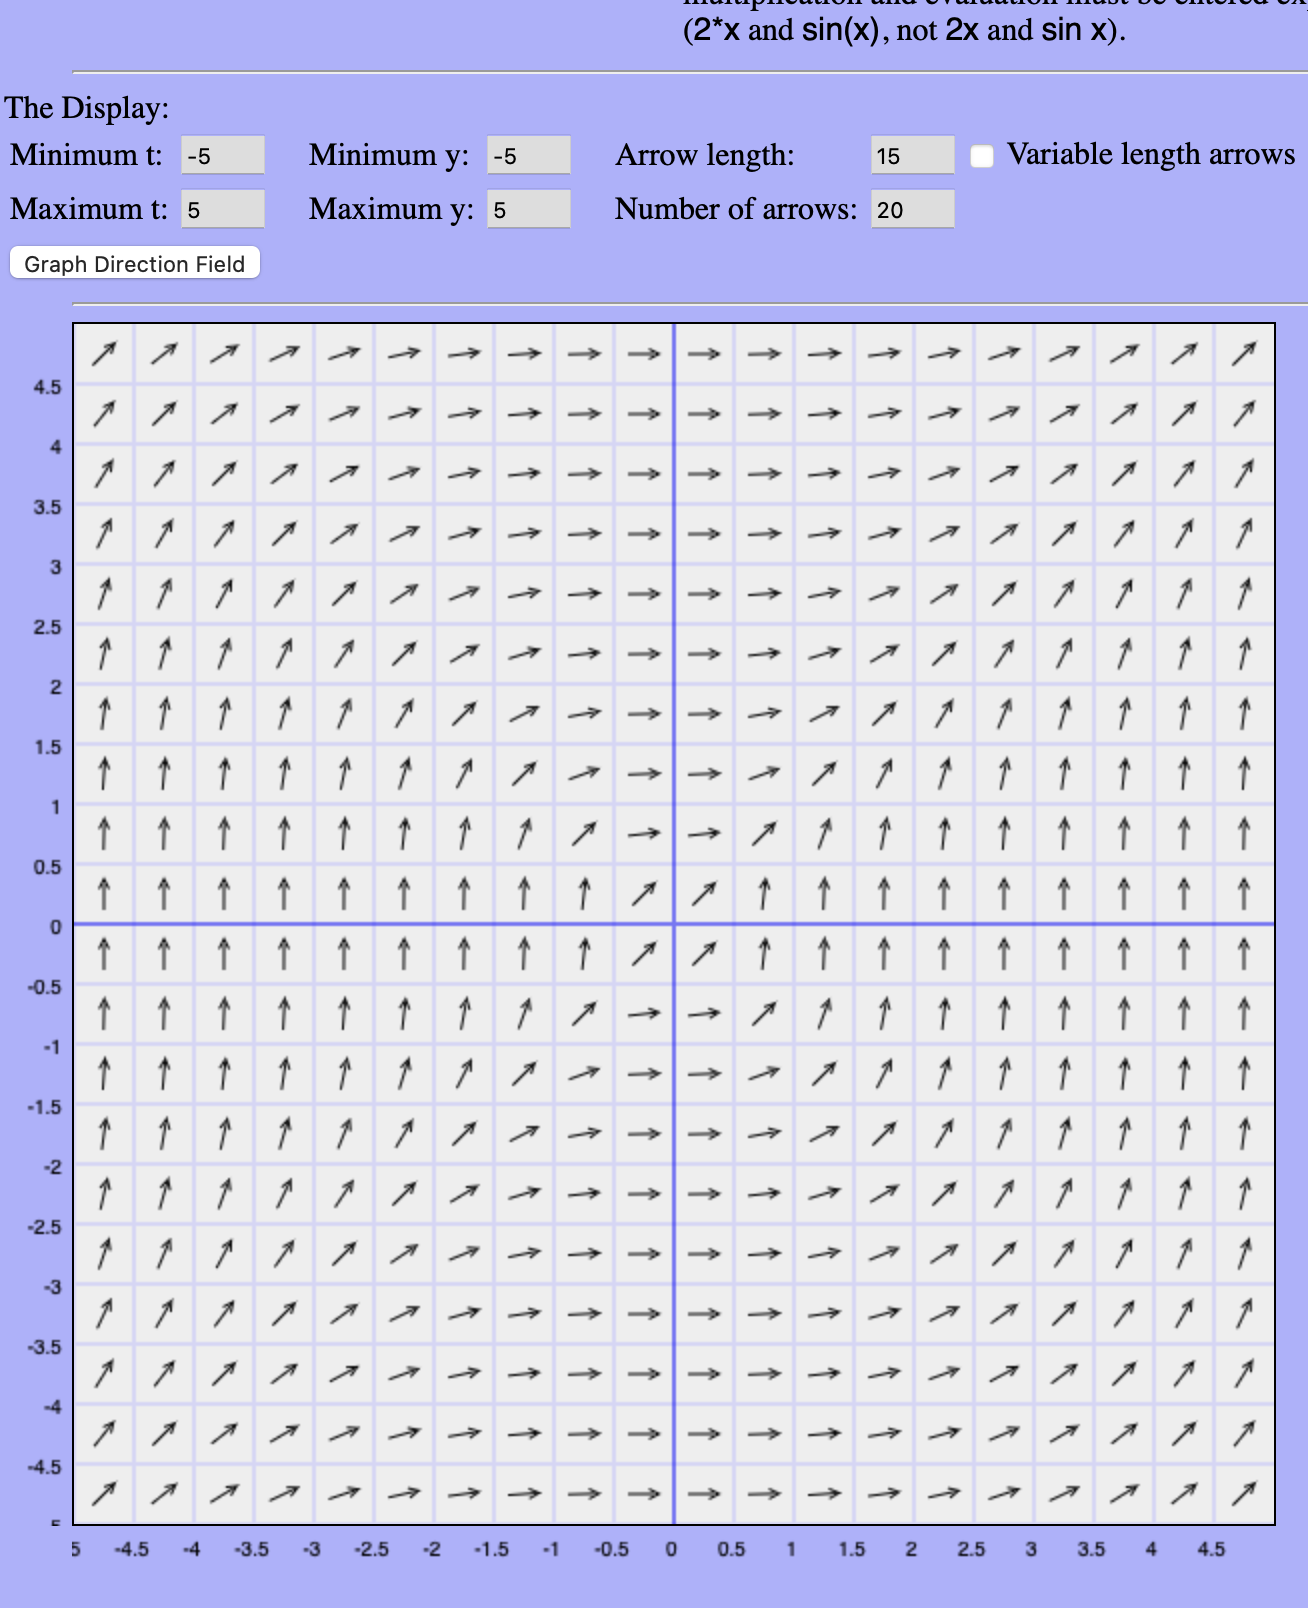
\includegraphics[width=\textwidth]{./images/x^2=y^2_unit_vector.png} \\
        \caption{unit arrow}
        \label{fig:ksdjfkjx}
    \end{subfigure}
    \begin{subfigure}[b]{0.4\textwidth}
        \centering
        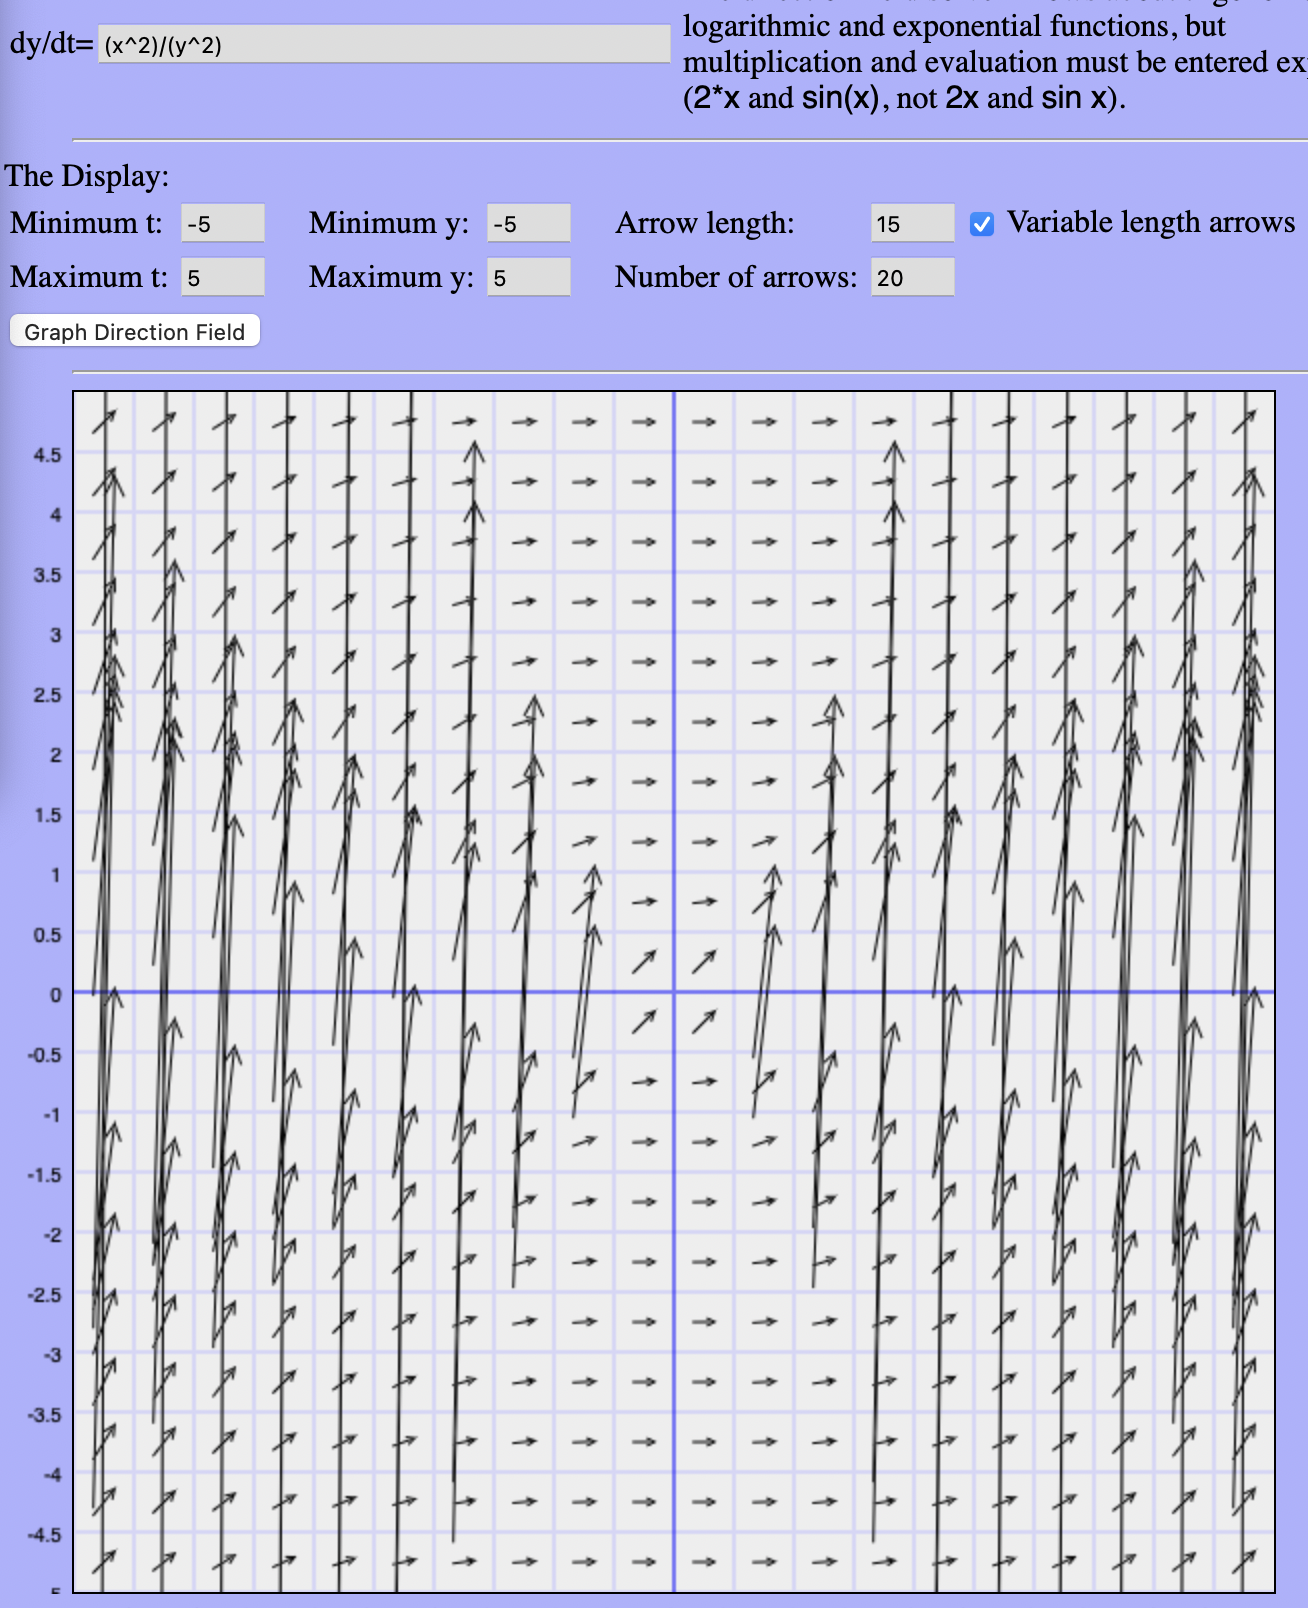
\includegraphics[width=\textwidth]{./images/x^2=y^2_arrow_length.png} \\
        \caption{Variable length arrow}
        \label{fig:xjsdfk x}
    \end{subfigure}
\end{figure}

% \import{exs/}{ex4.1.9.tex}
% \graphicspath{{./images/x^2=y^2.png}}

\end{document}
